\subsection{问题一原理}
\subsubsection{蒙特卡洛模拟方法}
\begin{defnbox}{蒙特卡洛模拟\cite{Weisstein2019monte}}{monte-carlo}
    通过生成合适的随机数并且观察符合某些属性来解决问题的方法称为蒙特卡洛模拟(或蒙特卡洛方法、随机抽样、统计试验方法)。
\end{defnbox}

网络上相关数据过少导致较难通过有监督的机器学习算法进行模型的训练,于是根据中国国内的真实数据进行数据建模,最后抽离出5个变量:城市机场密度、机场停机位数量、飞机时速、飞机客容量以及机场跑道容量。同时根据一定的规则(见附录~\ref{A:python-simulink}的\texttt{model\_airline.py}文),规划机场之间的航线,从而得到机场的客容量。根据实际情况进行建模,使用如图~\ref{fig:architecture}所视架构,共模拟中国45座城市、892条航线、14422架飞机,为解题提供充分的训练数据。

其中程序接口易用可拓展,整体架构清晰科学,并且数据格式统一,适合用来进行机器学习算法的训练。

\begin{figure}
    \centering
    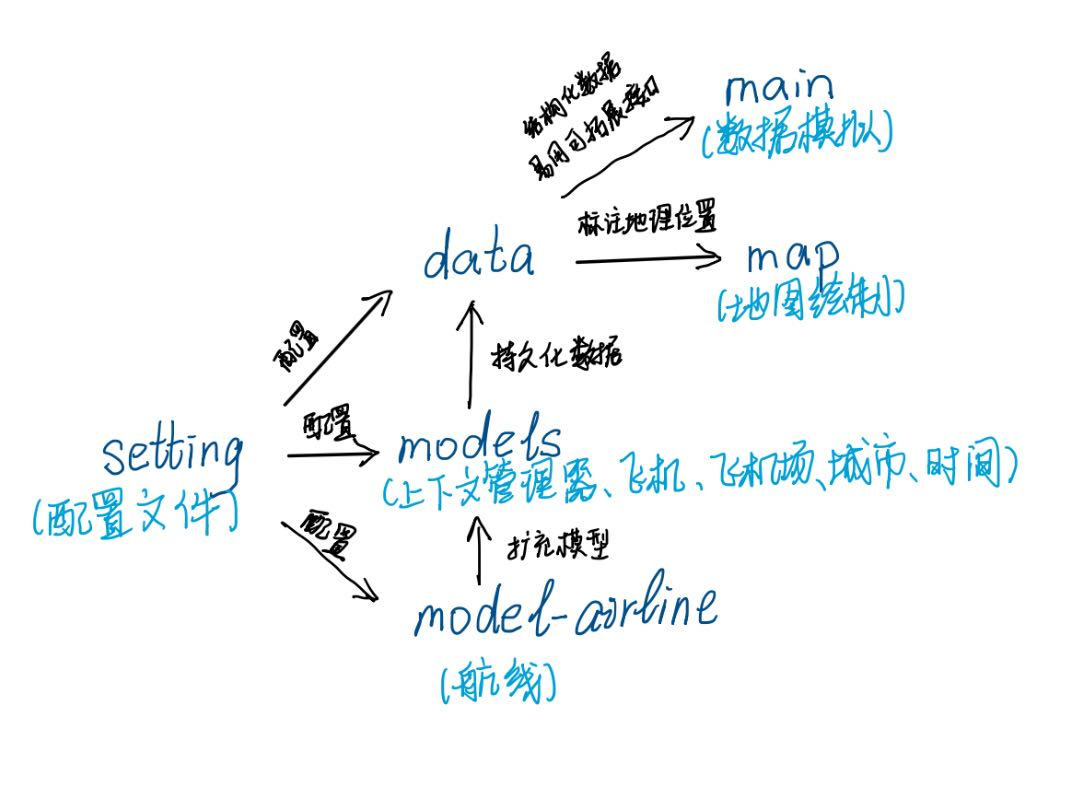
\includegraphics[width=.8\textwidth]{figures/程序架构.jpeg}
    \caption{程序架构}\label{fig:architecture}
\end{figure}


\subsection{问题一分析}
问题一旨在找出影响司机是否在机场选择载客的因素,即研究各因素与司机选择在机场载客返回市区的概率$P$的数量关系。

本文将影响因素拆分为乘客方面与司机方面两个角度。

\begin{enumerate}[label=(\arabic*)]
    \item 乘客方面,即潜在影响乘客选择出租车作为交通方式的因素分为三类:乘客到达时间段(即:乘客打车时段)$t$,乘客携带行李重量$m$,当时天气状况(即航班到达状态:延误/按时抵达)$weather$。由此三因素,进而影响当时乘客到达人数$N$及意愿选乘出租车的人数$N_p$。

    \item 司机方面,即影响司机选择在机场载客返回市区概率的因素为:乘客中意愿选乘出租车人数$N_p$,司机排队载客的平均等待时长$T$,司机的载客路程(即:机场至乘客目的地距离)$S_{out}$。
\end{enumerate}

同时使用中国范围内的直辖市、地级市、特别行政区、省会城市及各省其他主要知名城市的经纬度坐标,建立起``一城一港(北京机场设为两座航空港),两两相连''的飞行网络,见图~\ref{fig:path}。按照2018年旅客吞吐量,将我国机场大致分为四个梯队:

\begin{table}
    \centering
    \resizebox{\textwidth}{!}{%
        \begin{tabular}{ccccc}
            \hline
             & 第一梯队 & 第二梯队 & 第三梯队 & 第四梯队 \\ \hline
            \rowcolor[HTML]{EFEFEF}
            2018年旅客吞吐量 & >3000万 & 1000--3000万 & 200--1000万 & <200万 \\ \hline
        \end{tabular}%
    }
    \caption{中国机场分级依据}\label{T:classify_1}
\end{table}

蒙特卡罗模拟步骤具体如下:

\begin{enumerate}[label=(\arabic*)]
    \item 建立起“两两相连”的航空路线后,剔除始发机场与目的地机场间飞行时间短于30分钟的航线。
    
    如图\ref{fig:vector},$O$为始发港,设与其相关联的机场为$T_1$、$T_2$、$T_3$、$T_4$,已知四条航线距离$v_1$、$v_2$、$v_3$、$v_4$,根据余弦公式$\cos \theta_{ij} = |v_i\cdot v_j|/\left(|v_i|\cdot|v_j|\right)$, $i,j=1,\ldots,4$,可得出两两航空港地理位置间的夹角,夹角矩阵为$\Theta=\{\theta_{ij}\}_{i,j=1,\ldots,4} $运用离群值检验,得出临界夹角$\alpha$, $\ang{0.5}<\alpha<\ang{2}$,将$\theta$值小于$\alpha$的航线剔除。本图中,由于$O$港距$T_2$港过近且$\theta_{12}$较小,$v_2$航线可由$v_1$代替,故将$v_2$剔除。

\begin{figure}
    \centering
    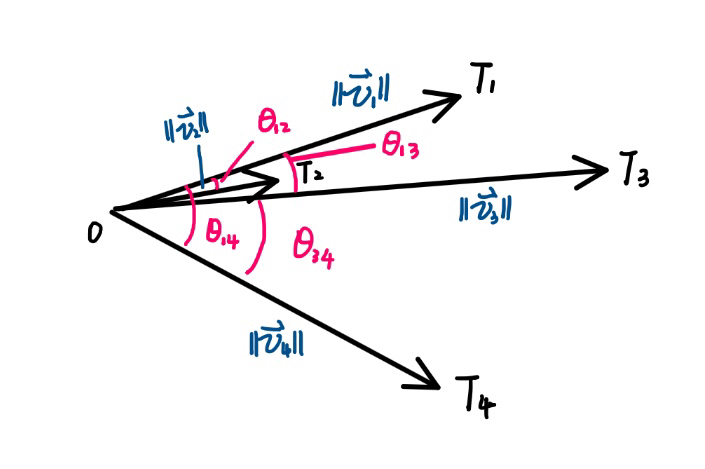
\includegraphics[width=.6\textwidth]{vector.jpg}
    \caption{飞机场节点剪枝策略}\label{fig:vector}
\end{figure}

    \item 将两地距离作为航线保留与否的权重,航线里程越长,权重越大,航线则越易被保留。计算上步剔除后各机场的节点数(即各机场的航线数),得到复杂矩阵$C_{1\times n}$,检查跨梯队间的机场是否仍存在航线联系,若存在,由于跨梯队间机场航线通常由同梯队联程航线代替,故剔除此类航线联系。
\end{enumerate}

% 航线877条
我国大陆三千万级以上机场的机位数及2018年旅客吞吐总量如表\ref{T:top10_num}所示:

\begin{table}
    \centering
    \resizebox{\textwidth}{!}{%
        \begin{tabular}{cccc}
            \hline
            IATA编号 & 机场名 & 机位数量(个) & 旅客吞吐量(万)(2018年) \\ \hline
            \rowcolor[HTML]{EFEFEF}
            XIY & 西安咸阳国际机场 & 127 & 4465 \\
            CTU & 成都双流国际机场 & 178 & 5291 \\
            \rowcolor[HTML]{EFEFEF}
            KMG & 昆明长水国际机场 & 110 & 4709 \\
            CKG & 重庆江北国际机场 & 209 & 4160 \\
            \rowcolor[HTML]{EFEFEF}
            SHA & 上海虹桥国际机场 & 155 & 4363 \\
            PVG & 上海浦东国际机场 & 218 & 7405 \\
            \rowcolor[HTML]{EFEFEF}
            CAN & 广州白云国际机场 & 220 & 6973 \\
            PEK & 北京首都国际机场 & 314 & 10098 \\
            \rowcolor[HTML]{EFEFEF}
            SZX & 深圳宝安国际机场 & 199 & 4935 \\
            HGH & 杭州萧山国际机场 & 127 & 3824 \\ \hline
        \end{tabular}%
    }
    \caption{中国大陆三千万级机场机位数及年旅客吞吐量}\label{T:top10_num}
\end{table}

 构建最直接影响$P$的因素与$P$间的数量关系,以多元线性关系为例:
 \begin{equation}\label{eq:linmodel}
    \begin{aligned}
        P &= \hat{N_p} + \beta_0 + \beta_1T + \beta_2S_{out} + \epsilon_t \\
          &= \gamma_0 + \delta_1t + \delta_2m + \delta_3weather + \beta_1T + \beta_2S_{out} + \eta_t
    \end{aligned}
\end{equation}

其中,$\beta_i$为待估计参数,$\eta_t$,$\epsilon_t$为白噪声误差项。由此,得出司机选择载客回市区的概率$P$。计算司机在此概率测度下的期望收益,即
\[
    E(\tilde{w}) = Pw_1 + (1-P)w_2,
\]
其中,$w_1$,$w_2$分别为司机载客所得收益及司机空载返回时的收益(为负)。
若$E(\tilde{w})>0$,则司机应选择等待载客,且此情况下应进一步优化策略使得$E(\tilde{w})$最大;若$E(\tilde{w})<0$,司机可选择空载返回市区。至此得到司机选择决策模型。
